\chapter{深度学习框架}\label{chap:framework}
\addtocontents{los}{\protect\addvspace{10pt}}

\begin{intro}
本章内容主要是对博客\textbf{The Anatomy of Deep Learning Frameworks}%
\footnote{https://medium.com/@gokul\_uf/the-anatomy-of-deep-learning-frameworks-46e2a7af5e47}%
的总结与整理。

可以考虑看看这个课程 CSE 599W: Systems for ML%
\footnote{http://dlsys.cs.washington.edu/}%
\end{intro}

许多初学者觉得深度学习框架抽象,虽然调用了几个函数/方法,计算了几个数学难题,
但始终不能理解这些框架的全貌。

为了更好地认识深度学习框架,也为了给一些想要自己亲手搭建深度学习框架的朋友提供
一些基础性的指导,日前来自苏黎世联邦理工学院计算机科学系的硕士研究生
Gokula Krishnan Santhanam在博客上撰文,概括了大部分深度学习框架都会包含
的五大核心组件,为我们详细剖析了深度学习框架一般性的内部组织结构。%
本文为雷锋网编译% TODO 在进行理解时,需要大量参考原英文博客,给了很多链接资料
\footnote{https://www.leiphone.com/news/201701/DZeAwe2qgx8JhbU8.html}%
。

Gokula Krishnan Santhanam认为,大部分深度学习框架都包含以下五个核心组件:
\begin{enumerate}
	\item 张量(Tensor)
	\item 基于张量的各种操作
	\item 计算图(Computation Graph)
	\item 自动微分工具(Automatic Differentiation)
	\item BLAS、cuBLAS、cuDNN 等扩展包
\end{enumerate}

\section{张量}\label{sec:tensor}

张量是所有深度学习框架中最核心的组件,因为后续的所有运算和优化算法都是基于张量进行的。
几何代数中定义的张量是基于向量和矩阵的推广,通俗一点理解的话,我们可以将标量视为零阶
张量,矢量视为一阶张量,那么矩阵就是二阶张量。

举例来说,我们可以将任意一张 RGB 彩色图片表示成一个三阶张量(三个维度分别是图片的高度、
宽度和色彩数据)。如图 \ref{} 所示,是一张普通的水果图片,按照 RGB 三原色表示,其
可以拆分为三张红色、绿色和蓝色的灰度图片,如果将这种表示方法用张量的形式写出来,就是
图中最下方的那张表格。

\begin{figure}[hbtp]
\centering
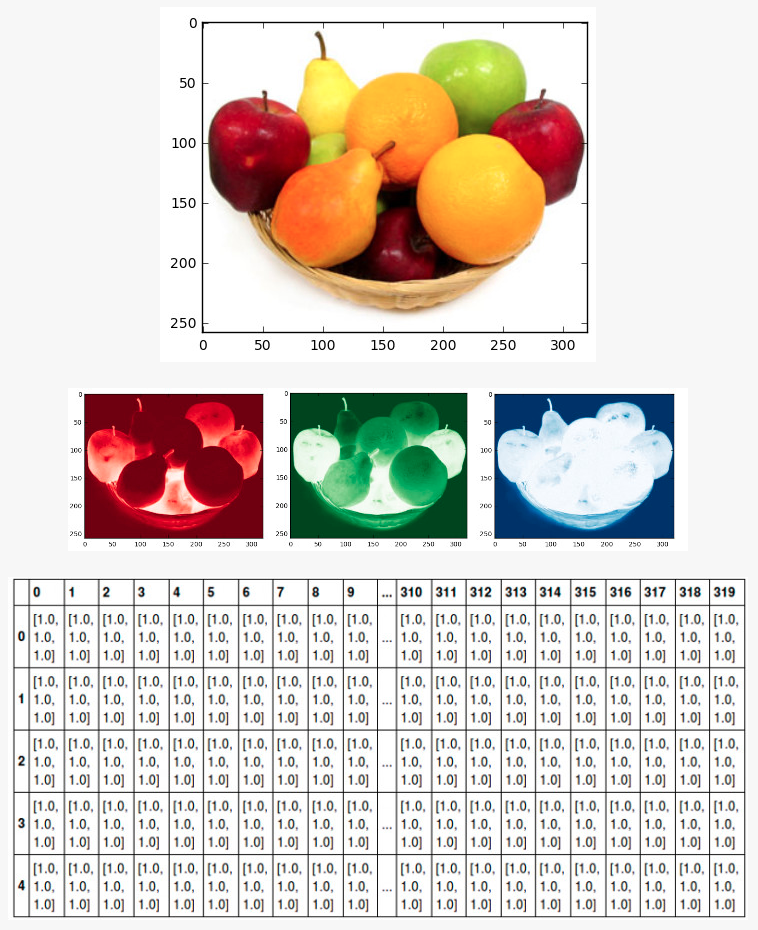
\includegraphics[width=0.45\textwidth]{framework-fruit-three-tensor}
\caption{水果的三种表示}
\label{fig:framework-fruit-three-tensor}
\end{figure}

图中只显示了前 5 行、320 列的数据,每个方格代表一个像素点,其中的数据 [1.0, 1.0, 1.0]
即为颜色。假设用[1.0, 0, 0]表示红色,[0, 1.0, 0]表示绿色,[0, 0, 1.0]表示蓝色,
那么前面5行的数据则全是白色。

将这一定义进行扩展,我们也可以用四阶张量表示一个包含多张图片的数据集,其中的四个维度分别是:
图片在数据集中的编号,图片高度、宽度,以及色彩数据。

将各种各样的数据抽象成张量表示,然后再输入神经网络模型进行后续处理是一种非常必要且高效的策略。
因为如果没有这一步骤,我们就需要根据各种不同类型的数据组织形式定义各种不同类型的数据操作,
这会浪费大量的开发者精力。更关键的是,当数据处理完成后,我们还可以方便地将张量再转换回
想要的格式。例如 Python Numpy 包中 numpy.imread 和 numpy.imsave 两个方法,分别
用来将图片转换成张量对象(即代码中的 Tensor 对象),和将张量再转换成图片保存起来。


\section{基于张量的各种操作}\label{sec:tensor-operations}

有了张量对象之后,下面一步就是一系列针对这一对象的数学运算和处理过程。如图 \ref{} 所示。

\begin{figure}[hbtp]
\centering
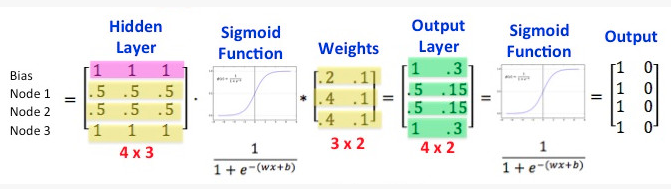
\includegraphics[width=0.85\textwidth]{framework-tensor-operations}
\caption{基于张量的各种操作}
\label{fig:framework-tensor-operations}
\end{figure}

其实,整个神经网络都可以简单视做为了达到某种目的,针对输入张量进行的一系列操作的过程。而所谓的
“学习”就是不断纠正神经网络的实际输出结果和预期结果之间误差的过程。这里的一系列操作包含的范围很宽,
可以是简单的矩阵乘法,也可以是卷积、池化和 LSTM 等稍复杂的运算。而且各框架支持的张量操作通常
也不尽相同,详细情况可以查看其官方文档。

需要指出的是,大部分的张量操作都是基于类实现的(而且是抽象类),而并不是函数(这一点可能要归功于
大部分的深度学习框架都是用面向对象的编程语言实现的)。这种实现思路一方面允许开发者将各种类似的操作
汇总在一起,方便组织管理。另一方面也保证了整个代码的复用性、扩展性和对外接口的统一。总体上让整个
框架更灵活和易于扩展,为将来的发展预留了空间。


\section{计算图}\label{sec:computation-graph}

有了张量和基于张量的各种操作之后,下一步就是将各种操作整合起来,输出我们需要的结果。

但不幸的是,随着操作种类和数量的增多,有可能引发各种意想不到的问题,包括多个操作之间应该并行还是
顺次执行,如何协同各种不同的底层设备,以及如何避免各种类型的冗余操作等等。这些问题有可能拉低整个
深度学习网络的运行效率或者引入不必要的Bug,而计算图正是为解决这一问题产生的。

计算图首次被引入人工智能领域是在 2009 年的论文《Learning Deep Architectures for AI》。
当时的示意图如下图 \ref{} 所示,作者用不同的占位符(*,+,sin)构成操作结点,以字母 x、a、b
构成变量结点,再以有向线段将这些结点连接起来,组成一个表征运算逻辑关系的清晰明了的“图”型数据结构,
这就是最初的计算图。

\begin{figure}[hbtp]
\centering
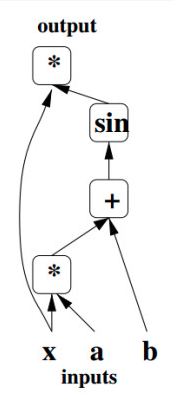
\includegraphics[width=0.25\textwidth]{framework-computation-graph}
\caption{最初的计算图}
\label{fig:framework-computation-graph}
\end{figure}

将计算图作为前后端之间的中间表示(Intermediate Representations)可以带来良好的交互性,
开发者可以将 Tensor 对象作为数据结构,函数/方法作为操作类型,将特定的操作类型应用于特定的
数据结构,从而定义出类似 MATLAB 的强大建模语言。

需要注意的是,通常情况下开发者不会将用于中间表示得到的计算图直接用于模型构造,因为这样的计算图
通常包含了大量的冗余求解目标,也没有提取共享变量,因而通常都会经过依赖性剪枝、符号融合、内存共享等
方法对计算图进行优化。

目前,各个框架对于计算图的实现机制和侧重点各不相同。例如 Theano 和 MXNet 都是以隐式处理的方式
在编译中由表达式向计算图过渡。而 Caffe 则比较直接,可以创建一个 Graph 对象,然后以类似
Graph.Operator(xxx) 的方式显示调用。

因为计算图的引入,开发者得以从宏观上俯瞰整个神经网络的内部结构,就好像编译器可以从整个代码的角度
决定如何分配寄存器那样,计算图也可以从宏观上决定代码运行时的 GPU 内存分配,以及分布式环境中不同
底层设备间的相互协作方式。除此之外,现在也有许多深度学习框架将计算图应用于模型调试,可以实时输出
当前某一操作类型的文本描述。


\section{自动微分工具}\label{sec:automatic-differentiation}

计算图带来的另一个好处是让模型训练阶段的梯度计算变得模块化且更为便捷,也就是自动微分法。

正如前面提到的,因为我们可以将神经网络视为由许多非线性过程组成的一个复杂的函数体,而计算图则以模块化
的方式完整表征了这一函数体的内部逻辑关系,因此微分这一复杂函数体,即求取模型梯度的方法就变成了在计算图
中简单地从输入到输出进行一次完整遍历的过程。与自动微分对应,业内更传统的做法是符号微分。

符号微分即常见的求导分析。针对一些非线性过程(如修正线性单元 ReLU)或者大规模的问题,使用符号微分法的
成本往往非常高昂,有时甚至不可行(即不可微)。因此,以上述迭代式的自动微分法求解模型梯度已经被广泛采用。
并且由于自动微分可以成功应对一些符号微分不适用的场景,目前许多计算图程序包
(例如Computation Graph Toolkit)都已经预先实现了自动微分。

另外,由于每个节点处的导数只能相对于其相邻节点计算,因此实现了自动微分的模块一般都可以直接加入任意的
操作类中,当然也可以被上层的微分大模块直接调用。


\section{BLAS/cuBLAS/cuDNN 等扩展包}\label{sec:blas-extension}

现在,通过上述所有模块,我们已经可以搭建一个全功能的深度学习框架:将待处理数据转换为张量,针对张量施加
各种需要的操作,通过自动微分对模型展开训练,然后得到输出结果开始测试。这时还缺什么呢?答案是运算效率。

由于此前的大部分实现都是基于高级语言的(如 Java、Python、Lua 等),而即使是执行最简单的操作,高级语言
也会比低级语言消耗更多的 CPU 周期,更何况是结构复杂的深度神经网络,因此运算缓慢就成了高级语言
的一个天然的缺陷。

目前针对这一问题有两种解决方案。

第一种方法是模拟传统的编译器。就好像传统编译器会把高级语言编译成特定平台的汇编语言实现高效运行一样,这种
方法将高级语言转换为 C 语言,然后在 C 语言基础上编译、执行。为了实现这种转换,每一种张量操作的实现代码
都会预先加入 C 语言的转换部分,然后由编译器在编译阶段将这些由 C 语言实现的张量操作综合在一起。目前
pyCUDA 和 Cython 等编译器都已经实现了这一功能。

第二种方法就是前文提到的,利用脚本语言实现前端建模,用低级语言如 C++ 实现后端运行,这意味着高级语言和
低级语言之间的交互都发生在框架内部,因此每次的后端变动都不需要修改前端,也不需要完整编译(只需要通过修改
编译参数进行部分编译),因此整体速度也就更快。

除此之外,由于低级语言的最优化编程难度很高,而且大部分的基础操作其实也都有公开的最优解决方案,因此另一个
显著的加速手段就是利用现成的扩展包。例如最初用 Fortran 实现的 BLAS(基础线性代数子程序),
就是一个非常优秀的基本矩阵(张量)运算库,此外还有英特尔的 MKL(Math Kernel Library)等,
开发者可以根据个人喜好灵活选择。

\begin{figure}[hbtp]
\centering
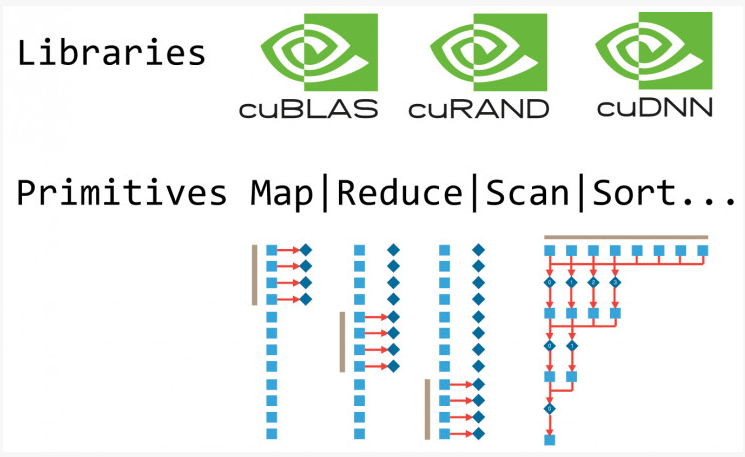
\includegraphics[width=0.5\textwidth]{framework-blas-extension}
\caption{BLAS/cuBLAS/cuDNN 等扩展包}
\label{fig:framework-blas-extension}
\end{figure}

值得一提的是,一般的 BLAS 库只是针对普通的 CPU 场景进行了优化,但目前大部分的深度学习模型都已经开始采用
并行 GPU 的运算模式,因此利用诸如 NVIDIA 推出的针对 GPU 优化的 cuBLAS 和 cuDNN 等更据针对性
的库可能是更好的选择。

运算速度对于深度学习框架来说至关重要,例如同样训练一个神经网络,不加速需要 4 天的时间,加速的话可能只要
4 小时。在快速发展的人工智能领域,特别是对那些成立不久的人工智能初创公司而言,这种差别可能就会决定谁是
先驱者,而谁是追随者。


\section{总结}\label{sec:framework-conclusion}

原文作者在文末指出:为了向开发者提供尽量简单的接口,大部分深度学习框架通常都会将普通的概念抽象化,这可能
是造成许多用户感知不到上述五点核心组件的重要原因。

而这也正是作者写本文的初衷:他希望开发者能够通过了解不同框架之间的一些相似特性,更好地认识和使用一个深度
学习框架。另一方面,对于那些不仅对学会使用深度学习框架感兴趣,还打算亲手搭建一个深度框架的朋友,作者认为
了解各框架的内部组成和一些共性的特征也是迈向成功的重要一步。他真诚地相信,一个优秀的工程师不仅应该
“知其然”,更应该“知其所以然”。


\endinput